\section{Content Analysis}
 
\subsection{Answer to RQ1 — How AI Mitigates Supply Chain Risks}
 
The analysis of the 19 included articles reveals six distinct mechanisms through which artificial intelligence is applied to mitigate risks in supply chains. Early warning and forecasting constitutes the dominant approach, identified in eight articles (42\%), followed by automation and decision support and resilience and recovery, each present in four articles (21\%). Privacy-preserving collaboration, explainability and transparency (XAI), and conceptual framework or review contributions each account for one article (5\%) respectively.
 
\begin{figure}[H]
  \centering
  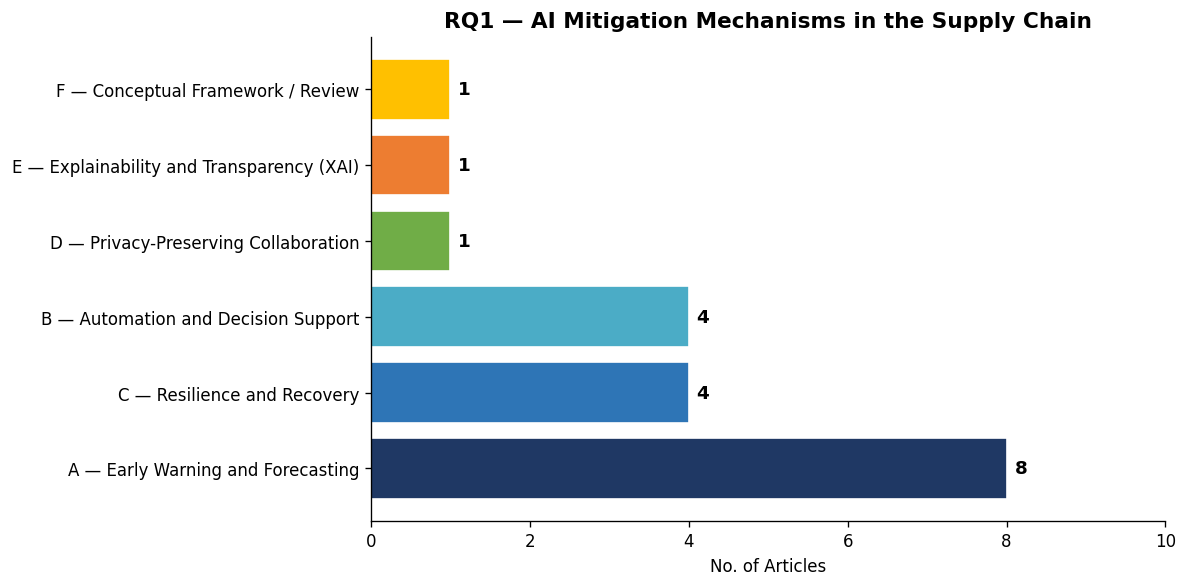
\includegraphics[width=\linewidth]{figures/fig_rq1_mitigation.png}
  \caption{Distribution of AI mitigation mechanisms across the 19 included articles (RQ1).}
  \label{fig:rq1}
\end{figure}
 
\textit{Early warning and forecasting} is the most pervasive mitigation mechanism in the literature, reflecting a theoretical consensus that preemptive anticipation of supply chain disruptions is more effective than post-event recovery. Studies in this category deploy AI models trained on historical operational and environmental data to generate alerts before risks materialise. Gradient boosting architectures (including LightGBM, XGBoost, and Random Forest) are applied to predict delayed deliveries and payment anomalies~\cite{adom2025design}, while deep learning frameworks combining GRU units, Bidirectional RNNs, and Transformer layers translate raw organisational data into probabilistic disruption forecasts~\cite{li2025endtoend}. Hybrid GNN-LSTM models capture both spatial supplier-relationship embeddings and temporal risk patterns simultaneously~\cite{farzhana2025hybrid}. Machine learning and data mining underpin a collaborative early warning system for China's manufacturing sector~\cite{yang2025design}, and knowledge graph-based frameworks integrate Graph Neural Networks and weakly supervised learning for risk monitoring, early warning, and decision support~\cite{yang2024building}. Real-time text mining and sentiment analysis applied to social media streams extend the early warning paradigm to unstructured data sources, enabling detection of emerging disruptions such as port congestion and semiconductor shortages as they develop~\cite{deivaganesh2022supply}. Review contributions document the broader transition from reactive to proactive risk management enabled by this class of AI application~\cite{deivaganesh2022future, le2025crisis}.
 
\textit{Automation and decision support} encompasses AI-driven systems that reduce human workload in risk-related decisions or automate responses to identified threats. Lin et al.~\cite{lin2025generative} introduce the UNISONE framework, which combines a Generative AI module for extracting disruption signals from unstructured text with Markov state modelling and Mixed Integer Programming for adaptive capacity reallocation. Explainable AI methods incorporating SHAP attribution and TOPSIS multi-criteria ranking automate and transparently support supplier selection decisions~\cite{kumar2023enhancing}. A multi-agent architecture integrating an LLM, an LSTM autoencoder, Random Forest, K-Means clustering, and Reinforcement Learning automates routing, anomaly detection, ESG scoring, and risk classification within a unified pipeline~\cite{rajesh2025smartops}. Clustering algorithms that segment suppliers into risk-performance profiles based on multiple operational indicators further exemplify AI-driven automation of vendor management decisions~\cite{gupta2025supplier}.
 
\textit{Resilience and recovery} captures studies that use AI to model, simulate, or support the restoration of supply chain continuity following disruption. Fernando et al.~\cite{fernando2024covid} examine how machine learning informs manufacturing firms' adaptive responses to COVID-19 disruption, while Nayal et al.~\cite{nayal2022exploring} investigate how AI adoption supports the agro-industry in sustaining operations under pandemic-induced supply chain stress. Nguyen et al.~\cite{nguyen2024federated} demonstrate how Federated Machine Learning enables collaborative risk prediction across supply chain partners to support network-level resilience, and Naz et al.~\cite{naz2022artificial} systematically document AI as an enabler of supply chain resiliency in the post-COVID-19 context.
 
\textit{Privacy-preserving collaboration} is addressed in one article. Nguyen et al.~\cite{nguyen2024federated} show that Federated Machine Learning allows supply chain partners to collaboratively train risk prediction models (combining CNN and LSTM components) without sharing proprietary raw data, resolving a fundamental barrier to multi-stakeholder AI adoption.
 
\textit{Explainability and transparency (XAI)} as a standalone mitigation mechanism is the focus of one systematic review. Nimmy et al.~\cite{nimmy2022explainability} comprehensively evaluate the suitability of XAI algorithms for supply chain operational risk management, establishing a methodological benchmark for transparent risk detection and positioning explainability as a first-class design requirement for applied AI in this domain.
 
\textit{Conceptual framework and review} contributions provide the theoretical scaffolding on which applied studies build. Aldehayyat et al.~\cite{aldehayyat2025applying} propose a digital transformation framework integrating AI and machine learning within an agile management paradigm, addressing the organisational prerequisites for AI-driven risk mitigation.
 
Overall, the dominance of early warning and forecasting reflects an underlying conviction in the literature that the most effective form of supply chain risk management is pre-emptive. The emergence of multi-agent and LLM-based architectures in 2025 articles suggests that the field is beginning to operationalise this logic at higher temporal resolution, moving from batch prediction toward continuous, automated risk surveillance.
 
% ----------------------------------------
 
\subsection{Answer to RQ2 — Types of Supply Chain Risks Addressed}
 
The cross-reference matrix produced from the 19 included articles reveals eight distinct risk type categories addressed through AI-based approaches: supplier risk, disruption risk, logistics and transport risk, demand and inventory risk, cybersecurity risk, pandemic risk, geopolitical risk, and fraud and integrity risk. Coverage is unequal across these categories, with logistics and transport risk and disruption risk attracting the highest number of AI technique applications, while cybersecurity, geopolitical, and fraud risks remain markedly under-represented.
 
\begin{figure}[H]
  \centering
  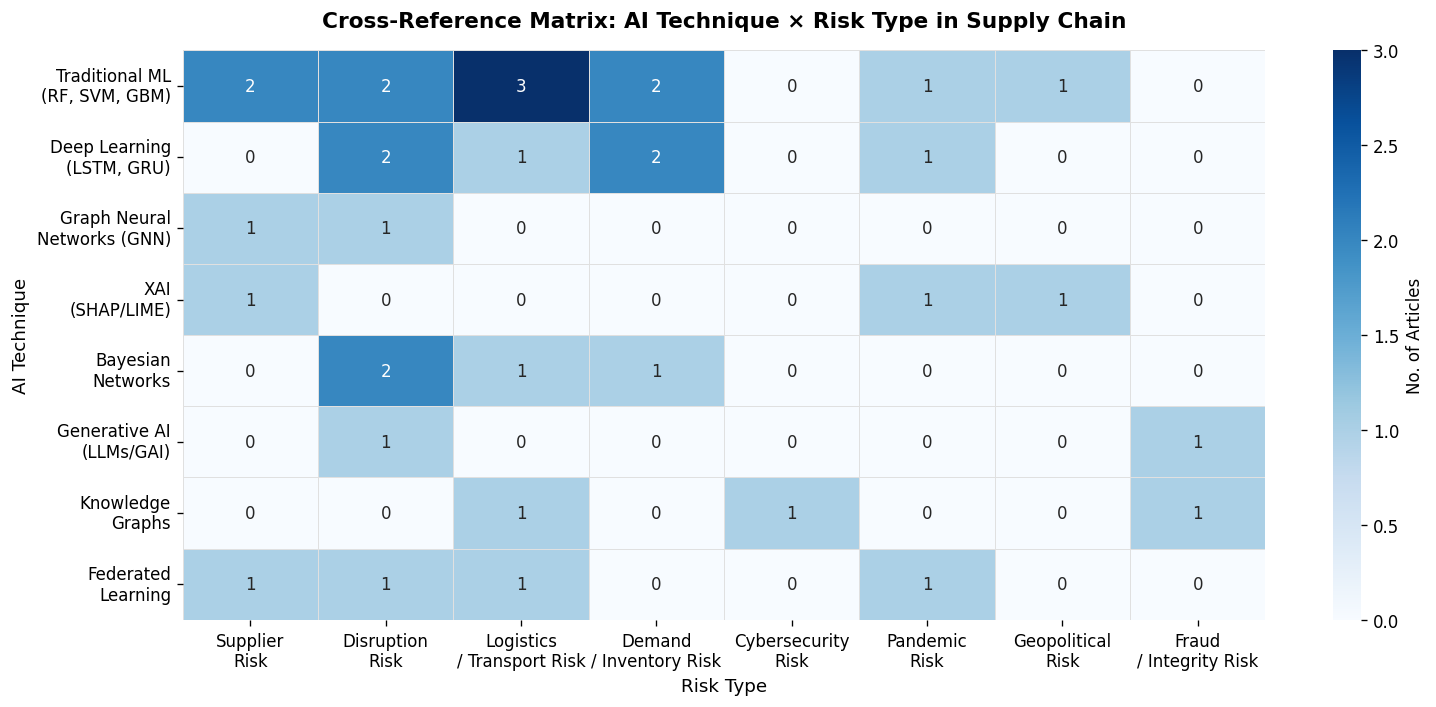
\includegraphics[width=\linewidth]{figures/fig_heatmap.png}
  \caption{Cross-reference matrix of AI techniques and supply chain risk types addressed in the included articles. Cell values indicate the number of articles addressing each combination.}
  \label{fig:heatmap}
\end{figure}
 
\textit{Logistics and transport risk} (encompassing transportation disruptions, port congestion, lead time variability, and distribution network failures) receives the broadest AI coverage across the corpus. Traditional machine learning methods (Random Forest, SVM, GBM) address this category in three articles, with additional coverage from Deep Learning, Bayesian Networks, Knowledge Graphs, and Federated Learning, reflecting the data richness and operational measurability of logistics processes~\cite{deivaganesh2022supply, yang2024building, nguyen2024federated}.
 
\textit{Disruption risk} is addressed by the widest range of AI technique categories (traditional ML, Deep Learning, Bayesian Networks, Generative AI, and Federated Learning), confirming it as the most cross-cutting risk type in the literature. This breadth reflects the scale of academic response to the COVID-19 pandemic and subsequent geopolitical instability, which exposed the fragility of global supply networks to macro-level shocks~\cite{li2025endtoend, lin2025generative, nguyen2024federated, fernando2024covid}.
 
\textit{Supplier risk} (covering supplier failure, quality issues, delivery delays, and credit default) is addressed predominantly through traditional ML methods and GNNs, which are particularly suited to modelling network-level interdependencies among suppliers~\cite{farzhana2025hybrid, yang2024building, kumar2023enhancing}.
 
\textit{Demand and inventory risk}, arising from demand volatility, forecast errors, and inventory misalignment, is addressed by traditional ML and Deep Learning in two articles each, reflecting the long-standing application of statistical learning to demand forecasting problems~\cite{adom2025design, li2025endtoend}.
 
\textit{Pandemic risk} receives dedicated attention in three articles through traditional ML, XAI, and Federated Learning, confirming the COVID-19 pandemic as a structuring event for this research stream~\cite{nayal2022exploring, nimmy2022explainability, nguyen2024federated}.
 
\textit{Geopolitical risk} is addressed in two articles through traditional ML and XAI-based approaches~\cite{aldehayyat2025applying, kumar2023enhancing}. \textit{Fraud and integrity risk} appears in two articles deploying Generative AI and Knowledge Graphs~\cite{lin2025generative, yang2024building}. \textit{Cybersecurity risk} is the least studied category, identified in only one article through a Knowledge Graph-based approach~\cite{yang2024building}, representing a critical gap given the increasing digitalisation of supply chain operations.
 
 
\subsection{Answer to RQ3 — AI Techniques Used}
 
The methodological landscape of the 19 included articles encompasses eight distinct AI technique categories. Traditional machine learning (comprising Random Forest, Support Vector Machines, and Gradient Boosting Methods) is the most widely deployed category, applied across the broadest range of risk types. Deep Learning (LSTM, GRU), Graph Neural Networks (GNN), XAI (SHAP/LIME), Bayesian Networks, Generative AI (LLMs), Knowledge Graphs, and Federated Learning constitute the remaining categories, reflecting a methodologically diverse corpus.
 
\textit{Traditional machine learning} (Random Forest, SVM, GBM) addresses supplier risk (2 articles), disruption risk (2 articles), logistics and transport risk (3 articles), demand and inventory risk (2 articles), pandemic risk (1 article), and geopolitical risk (1 article), demonstrating the broadest risk coverage of any single technique category~\cite{adom2025design, aldehayyat2025applying, yang2025design, gupta2025supplier}. The versatility of these methods for structured, tabular supply chain data explains their continued prevalence despite the emergence of more complex architectures.
 
\textit{Deep Learning} (LSTM, GRU) is applied to disruption risk (2 articles), logistics and transport risk (1 article), demand and inventory risk (2 articles), and pandemic risk (1 article)~\cite{li2025endtoend, farzhana2025hybrid}. The temporal modelling capabilities of recurrent architectures make them particularly suited to supply chain time-series data, where historical sequences encode the dynamics of disruption propagation.
 
\textit{Graph Neural Networks} address supplier risk (1 article) and logistics and transport risk (1 article)~\cite{yang2024building, farzhana2025hybrid}, reflecting the natural fit between graph-structured models and the network topology of supply chains, where risks propagate through supplier-buyer relationships.
 
\textit{XAI (SHAP/LIME)} is applied to supplier risk (1 article), pandemic risk (1 article), and geopolitical risk (1 article)~\cite{kumar2023enhancing, nimmy2022explainability}, confirming the growing importance of interpretability as a design requirement for AI systems deployed in high-stakes supply chain decisions.
 
\textit{Bayesian Networks} address disruption risk (2 articles), logistics and transport risk (1 article), and demand and inventory risk (1 article)~\cite{deivaganesh2022future, naz2022artificial}, providing probabilistic modelling capabilities well-suited to uncertainty quantification under incomplete information.
 
\textit{Generative AI (LLMs)} appears in two articles addressing disruption risk and fraud and integrity risk~\cite{lin2025generative, rajesh2025smartops}, representing the most recent technical development in the corpus and signalling the entry of large language model capabilities into supply chain risk management.
 
\textit{Knowledge Graphs} address logistics and transport risk (1 article), cybersecurity risk (1 article), and fraud and integrity risk (1 article)~\cite{yang2024building}, offering structured knowledge representation capabilities for complex, multi-entity risk environments.
 
\textit{Federated Learning} addresses supplier risk (1 article), disruption risk (1 article), logistics and transport risk (1 article), and pandemic risk (1 article)~\cite{nguyen2024federated}, enabling privacy-preserving collaborative risk modelling across organisational boundaries.
 
A temporal trend is discernible: articles published in 2022 and 2023 predominantly rely on traditional ML and review-based methods, while 2024 and 2025 contributions increasingly deploy hybrid architectures combining Deep Learning, GNNs, Generative AI, and formal optimisation. The appearance of LLMs in two 2025 articles suggests that generative AI capabilities are beginning to be operationalised for supply chain risk management, a trend likely to intensify as domain-specific model fine-tuning becomes more accessible.
  
\subsection{Complementary Analysis}
 
\textit{Sector concentration.} The majority of included articles propose general or sector-agnostic supply chain models, limiting the ability to draw sector-specific conclusions. Where specific industries are targeted, manufacturing receives the most attention~\cite{yang2025design, li2025endtoend}, followed by logistics and transportation~\cite{le2025crisis, rajesh2025smartops}, agriculture~\cite{nayal2022exploring}, e-commerce and contract logistics~\cite{adom2025design}, and multi-sector contexts including pharmaceuticals, food, and semiconductors~\cite{lin2025generative}. Healthcare, energy, and public sector supply chains are absent from the corpus, representing sectors where AI-based risk management frameworks remain underdeveloped.
 
\textit{Geographic distribution.} Indian institutions are affiliated with six articles~\cite{deivaganesh2022future, deivaganesh2022supply, farzhana2025hybrid, gupta2025supplier, naz2022artificial, rajesh2025smartops}, constituting the most active national research community in the corpus. China contributes two articles~\cite{yang2024building, yang2025design} and Vietnam two articles~\cite{le2025crisis, nguyen2024federated}, with the remaining studies originating from multi-institutional collaborations across Taiwan, Japan, Jordan, the United Kingdom, France, and Brazil. Primary contributions from North America and continental Europe are absent, despite these regions' substantial supply chain research traditions.
 
\textit{Temporal evolution.} Publication volume increases steadily from two articles in 2022 to four in 2025, with one article already slated for 2026, confirming a clear upward trajectory. The COVID-19 pandemic serves as the principal inflection point, with the most technically sophisticated contributions (deploying LLMs, multi-agent systems, and advanced hybrid architectures) concentrated in 2025.